\documentclass[a3paper,landscape,11pt,fleqn]{article}%fleqn pour aligner les equations à gauche
\usepackage{../../Styles/Cours}

\newcommand{\chnum}{Chapitre 15}
\newcommand{\chtitle}{Lumière et spectres}
\newcommand{\dtype}{Cours}
\usepackage{hyperref}

\begin{document}
	\maketitle
\begin{multicols}{2}	
	\section*{Partie 1 : La lumière}
	\begin{minipage}{\linewidth}
	\begin{center} \textbf{Document 1 : Plein les yeux} \end{center}
		L’Homme depuis la nuit des temps n’a eu comme seul attribut pour observer le monde que son œil nu. Par les nuits les plus noires, il ne pouvait compter que sur la lumière des étoiles pour ce repérer. C’est pourquoi il a rapidement su exploiter l’incandescence.\\
		Lorsqu’il est convenablement chauffé, le bois prend feu et la flamme qui en résulte crée un halo de lumière. Des siècles plus tard, le filament d’une lampe portée à incandescence éclaire alors ses nuits. La lumière des étoiles nous permet de distinguer la lueur rouge de Bételgeuse (une étoile dont la température de surface est de l’ordre de \SI{3000}{\celsius}), ou l’éclat bleuté de Rigel (avec une température de surface de plus de \SI{11000}{\celsius}). Entre les deux, notre Soleil, jaune affiche à sa surface une température de \SI{5000}{\celsius}.
		\label{fig:doc1}
	\end{minipage}
	\begin{enumerate}
		\item Quelles sont les sources lumineuses citées dans le texte ?
		\item Quelles hypothèses pouvez vous émettre pour expliquer les couleurs différentes des rayons lumineux émis par les étoiles ?
	\end{enumerate}
	
	
		\begin{center}\textbf{Document 2 : Orion le chasseur} \end{center}
		\begin{minipage}{.24\textwidth}
			Les étoiles apparaissent être exclusivement blanches au premier coup d’œil. Mais si nous regardons attentivement, nous pouvons noter une plage de couleurs : bleu, blanc, rouge et même doré. Dans la constellation d’hiver d’Orion, un beau contraste se voit entre la rouge Bételgeuse et la bleue Bellatrix. Ce qui fait que les étoiles montrent différentes couleurs resta longtemps un mystère jusqu’à il y a deux siècles, quand les physiciens eurent suffisamment de compréhension de la nature de la lumière et des propriétés de la matière aux très hautes températures.\\
			Les étoiles sont très éloignée de nous, à un tel point que la lumière qu'elles émettent mettent plusieurs années à vous parvenir. Par exemple la lumière émise par l’étoile Bételgeuse met environ 643 années pour nous parvenir.
		\end{minipage}\hspace{2em}
		\begin{minipage}{.2\textwidth}
			\centering 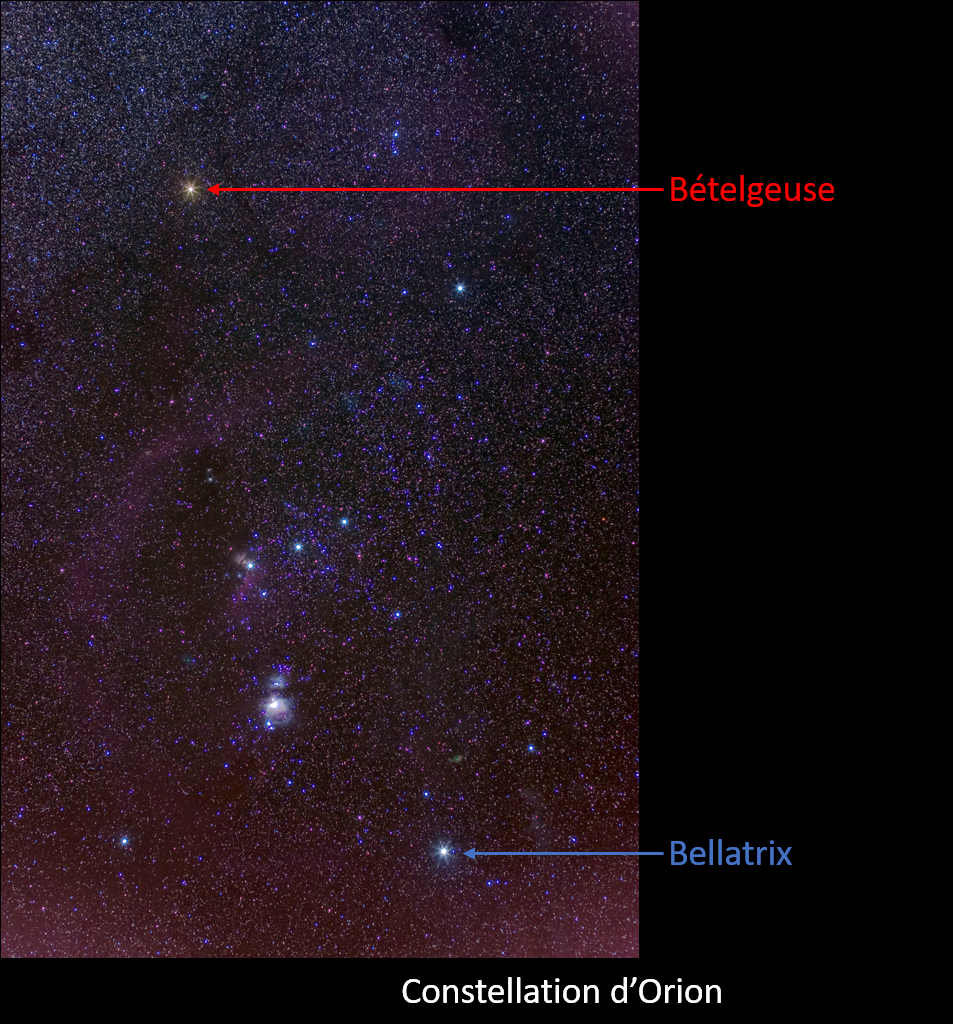
\includegraphics[width=\linewidth]{Ressources/Act1_fig1.png}
		\end{minipage}
		\label{fig:doc2}

	\begin{enumerate}[resume]
		\item Sachant que la lumière se déplace dans le vide à une vitesse d'environ \SI{299792458}{\meter\per\second}, à quelle distance se situe Bételgeuse ?
	\end{enumerate}
	
	\begin{cours}
		Les ondes électromagnétiques, dont la lumière fait partie, se propagent toutes à la même vitesse dans le vide ou dans l'air. Cette vitesse notée $c$ a pour valeur exacte \SI{299792458}{\meter\per\second}. On reviendra la valeur arrondie : $c=\SI{3,00E8}{\meter\per\second}$.
	\end{cours}
	

	\section*{Partie 2 : L'émission de lumière}
	\textbf{Pourquoi les étoiles n'ont pas la même couleur ? Comment peut-on analyser la lumière qui vous vient des étoiles ?}
	
	\begin{enumerate}
		\item Pourquoi ne peut-on pas effectuer une étude \emph{in situ} de la composition du Soleil en envoyant une sonde par exemple ?
		\item Sur quel phénomène physique peut on alors s'appuyer ?
		\item De quels moyens techniques disposons-nous pour l"analyser ?
	\end{enumerate}
	\subsection{Décomposition de la lumière : le spectre continu émis par une lampe à incandescence}
	\begin{figure}[h!]
		\centering
		\caption*{Schéma du montage}
		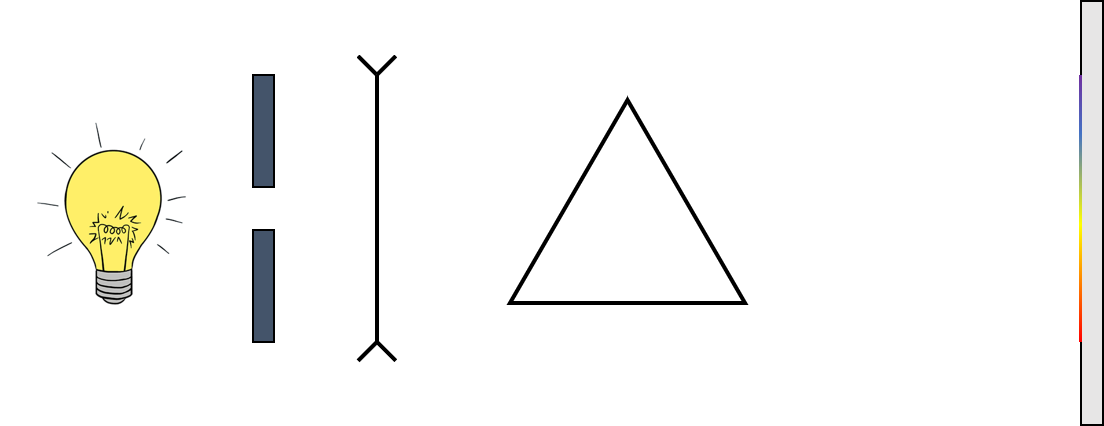
\includegraphics[width=.4\linewidth]{Ressources/Act1_fig2.png}
		\label{fig:doc3}
	\end{figure}
	
	\begin{enumerate}[resume]
		\item Compléter et légender le schéma du montage
		\item Décrire le phénomène que vous observez
	\end{enumerate}
	
	\begin{enumerate}[resume]
		\item Quelles sont les limites du spectre visible de la lumière blanche ?
		\item Que signifient les termes "UV" et "IR" ?
	\end{enumerate}
	\begin{figure}[h!]
		\centering
		\caption*{Spectre visible de la lumière blanche}
		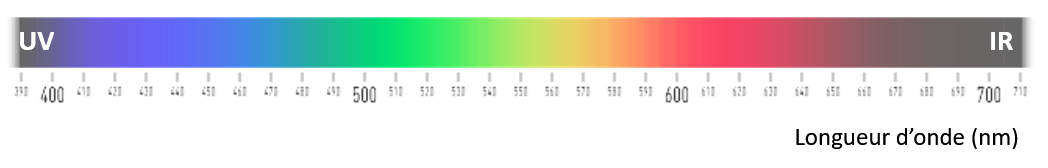
\includegraphics[width=.8\linewidth]{Ressources/Act1_fig3.png}
		\label{fig:doc4}
	\end{figure}
	\begin{cours}
			La lumière émise par l'ampoule peut être décomposée par ....................... On obtient alors un ....................... montrant un étalement de couleur du ....................... au .......................\\
			La lumière est constituée de ....................... Chacune d'entre elle est caractérisée par une ....................... notée $\lambda$ (lambda) exprimé en \textbf{nanomètre} (\unit{\nano\meter}). Pour décomposer la lumière, on utilise un ....................... (\textbf{prisme ou réseau} qui permet d'obtenir, sur l'écran, une figure appelée .......................\\
			L'\oe il humais n'est capable d'observer qu'une petite partie du spectre lumineux, il s'agit de la lumière visible comprenant des radiations allant de \num{400} à \SI{800}{nm}.\\
			
			\begin{tikzpicture}[scale=.9,transform shape]
				\draw (0,0) -- (18,0)--(18,1)--(0,1) --cycle;
				\draw (0.75,0)--(0.75,1);
				\draw (1.5,0)--(1.5,1);
				\draw (6,0)--(6,1);
				\draw (6.75,0)--(6.75,1);
				\draw (9,0)--(9,1);
				\draw[-stealth,thick] (0,-2) to (18.5,-2);
				\foreach \k in {1,...,24} {
					\pgfmathsetmacro\result{0.75*\k}
					\draw (\result, -2) -- (\result, -1.5);
				};
				\draw (0,-1.75) node[left]{\huge $\mathbf{\lambda}$};
			\end{tikzpicture}
		\end{cours}
		
		\subsection{Spectre d'émission des corps chauds}
		\begin{minipage}{.48\linewidth}
			Pour étudier l'effet de la température d'un corps lorsqu'il est chauffé on utilise un simulateur permettant de faire varier la température d'on objet et affichant le spectre et la couleur de la lumière associée.\\
			\url{https://phet.colorado.edu/sims/html/blackbody-spectrum/latest/blackbody-spectrum_all.html?locale=fr}
		\end{minipage}\hspace{2em}
		\begin{minipage}{.48\linewidth}
			\centering 
\includegraphics[width=.5\linewidth]{Ressources/qR_PHET_Corps_chaud.png}
		\end{minipage}	
		
		\begin{table}[h!]
			\centering
			\caption*{Résumé de la simulation}
			\begin{tabular}{|>{\centering}m{.2\linewidth}|>{\centering}m{.2\linewidth}|>{\centering}m{.2\linewidth}|>{\centering\arraybackslash}m{.2\linewidth}|}\hline
				Température & Mini & & Maxi\\ \hline
				Valeur en Kelvin& & & \\ \hline
				Valeur du pic du spectre& & & \\ \hline
				Couleur observable& & & \\ \hline
			\end{tabular}
			\label{tab:tableau}
		\end{table}
		\begin{enumerate}
			\item Comment évolue la température du filament de la lampe lorsque l'intensité qui la traverse augmente ?
			\item Que peut-on en conclure sur le spectre lumineux d'un corps fortement chauffé ?
		\end{enumerate}
		
		\noindent\fbox{\begin{minipage}{\linewidth}
				\textbf{Cours :}\\
				Un corps fortement chauffé émet de la lumière dont le spectre est ....................... Ce spectre ne dépend pas de la composition du corps. En revanche, il dépend de sa .......................\\
				Lorsque la température du corps ......................., la lumière qu'il émet s'enrichit en radiations .............................................. : son spectre continu d'émission s'étale d'avantage vers le .......................
		\end{minipage}}
		
		\subsection{Spectres de raies d'émission d'un gaz}
		Le professeur branche la lampe spectrale à vapeur de sodium puis celle au mercure. Observer la lampe à travers un spectroscope.
		\begin{enumerate}
			\item Faire un schéma du montage et reproduire les spectres d'émission observés.
		\end{enumerate}
		\begin{figure}[h!]
			\centering
			\caption*{Schéma du montage}
			\begin{tikzpicture}
				\draw (0,0) rectangle(18,4);
			\end{tikzpicture}
			\label{fig:enter-label}
		\end{figure}
		\begin{figure}[h!]
			\centering
			\caption*{Spectre d'émission de la lampe à vapeur de sodium}
			\begin{tikzpicture}
				\draw (0,0) rectangle(15,2);
				\foreach \k in {0,...,15} {
					\draw (\k,-.25)--(\k,.25);
				};
				\foreach \k in {0,5,10,15} {
					\pgfmathtruncatemacro\result{400 +20*\k}
					\draw[very thick] (\k,-.35)--(\k,.35);
					\draw (\k,-.35) node[below] {$\result$};
				};
			\end{tikzpicture}
			\label{fig:enter-label}
		\end{figure}
		\begin{figure}[h!]
			\centering
			\caption*{Spectre d'émission de la lampe à vapeur de mercure}
			\begin{tikzpicture}
				\draw (0,0) rectangle(15,2);
				\foreach \k in {0,...,15} {
					\draw (\k,-.25)--(\k,.25);
				};
				\foreach \k in {0,5,10,15} {
					\pgfmathtruncatemacro\result{400 +20*\k}
					\draw[very thick] (\k,-.35)--(\k,.35);
					\draw (\k,-.35) node[below] {$\result$};
				};
			\end{tikzpicture}
			\label{fig:enter-label}
		\end{figure}
		
		\begin{enumerate}[resume]
			\item Pourquoi décrit-on ce spectre comme un spectre de raies ?
			\item Les spectres d'émission dépendent-ils de l'élément chimique mis en jeu ?
		\end{enumerate}
		
		\noindent\fbox{\begin{minipage}{\linewidth}
				\textbf{Cours :}\\
				Un gaz porté à haute température sous une faible pression peut émettre de la lumière composée d'une ou de plusieurs ....................... Le spectre lumineux est alors ......................., il est appelé ..............................................
		\end{minipage}}
\end{multicols}
	\end{document}